\documentclass[sigconf]{acmart}
\usepackage[slantfont,boldfont]{xeCJK}
\setCJKmainfont{SimSong}

%%
%% \BibTeX command to typeset BibTeX logo in the docs
\AtBeginDocument{%
  \providecommand\BibTeX{{%
    \normalfont B\kern-0.5em{\scshape i\kern-0.25em b}\kern-0.8em\TeX}}}

%%
%% end of the preamble, start of the body of the document source.
\begin{document}

%%
%% The "title" command has an optional parameter,
%% allowing the author to define a "short title" to be used in page headers.
\title{机器学习在协同过滤和基于内容推荐中的应用}

%%
%% The "author" command and its associated commands are used to define
%% the authors and their affiliations.
%% Of note is the shared affiliation of the first two authors, and the
%% "authornote" and "authornotemark" commands
%% used to denote shared contribution to the research.

\author{尹祥琨}
\orcid{0000-0001-6417-0859}
\affiliation
{
  \institution{山东大学}
  \city{青岛}
  \country{中国}
}
\email{201805130154@mail.sdu.edu.cn}

%%
%% The abstract is a short summary of the work to be presented in the
%% article.
\begin{abstract}
  随着在线信息的数量、复杂性的不断增长,推荐系统已成为信息过载的关键解决方案。机器学习在语音识别、图像分析和自然语言处理方面的革命性进展引起了广泛关注。同时,早期研究工作也证明了机器学习在处理信息检索和推荐任务方面的有效性。凭借其高质量的推荐,将机器学习技术应用于推荐系统有开阔的前景。根据前人工作总结,推荐系统产生推荐列表的方式通常有三种:协同过滤以及基于内容推荐和这两种方法的混合模型。本文探究了机器学习在前两种不同类别推荐系统中的应用。
\end{abstract}

%%
%% The code below is generated by the tool at http://dl.acm.org/ccs.cfm.
%% Please copy and paste the code instead of the example below.
%%
\begin{CCSXML}
  <ccs2012>
     <concept>
         <concept_id>10002951.10003317.10003347.10003350</concept_id>
         <concept_desc>Information systems~Recommender systems</concept_desc>
         <concept_significance>500</concept_significance>
         </concept>
   </ccs2012>
\end{CCSXML}
  
\ccsdesc[500]{Information systems~Recommender systems}

%%
%% Keywords. The author(s) should pick words that accurately describe
%% the work being presented. Separate the keywords with commas.
\keywords{推荐系统, 机器学习}

%% A "teaser" image appears between the author and affiliation
%% information and the body of the document, and typically spans the
%% page.

\begin{teaserfigure}
  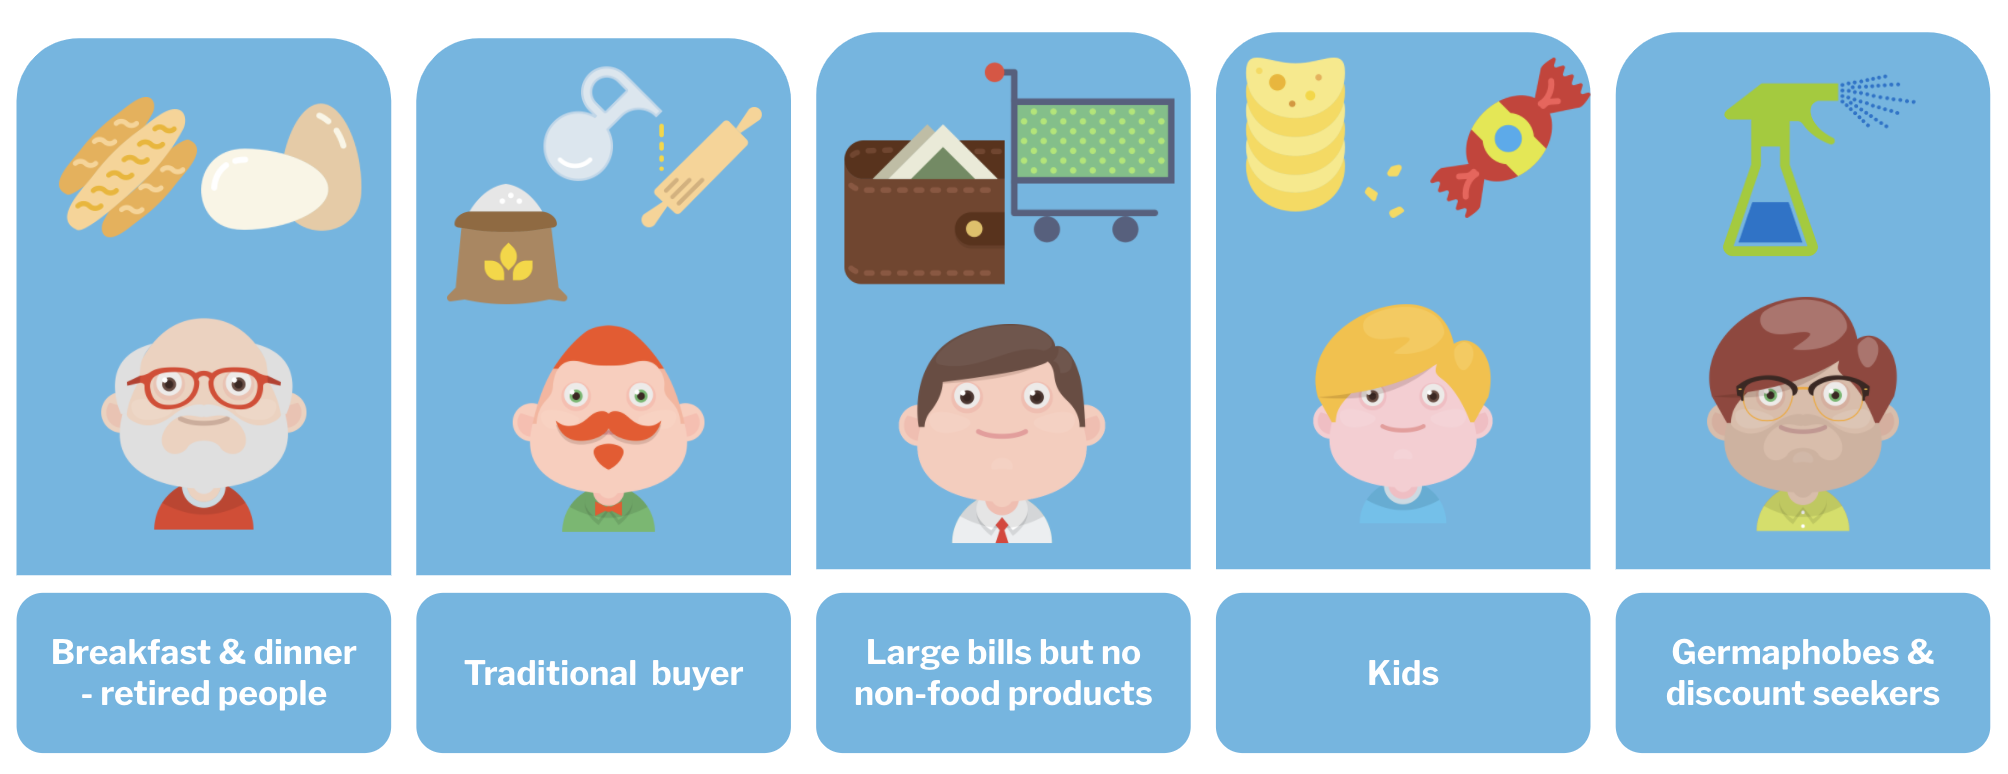
\includegraphics[width=\textwidth]{img/teaser.png}
  \caption{推荐系统是一种信息过滤系统,用于预测不同用户对物品的“偏好”。}
  \Description{针对不同人的喜好进行推荐}
  \label{fig:teaser}
\end{teaserfigure}

%%
%% This command processes the author and affiliation and title
%% information and builds the first part of the formatted document.
\maketitle

\section{Introduction}

信息时代下互联网信息量的爆炸式增长使用户目不暇接。推荐系统作为一种有效的信息过滤工具,用于指导用户以个性化的方式从大量可能的选项中发现他们可能感兴趣的产品或服务。推荐系统在各种信息访问系统中发挥着越来越重要的作用,以促进业务发展并促进决策过程。自上世纪90年代第一篇关于协同过滤的论文出现以来,推荐系统便成为一个重要的研究领域 \cite{hill1995recommending, resnick1994grouplens, shardanand1995social}。 在过去的十年中,工业界和学术界虽然在推荐系统的新方法方面已经做了很多工作,而对这一领域的兴趣仍保持高涨,因为推荐系统构成了一个问题丰富的研究领域,并且大量的实际应用程序可以帮助用户处理信息过载并为他们提供个性化的推荐、内容和服务。 常见的应用比如推荐Amazon上的书籍、CD 和其他产品、MovieLens上的电影等等。

过去几十年见证了机器学习(ML)在计算机视觉和语音识别等许多应用领域取得的巨大成功。学术界和工业界一直在竞相将机器学习应用于更广泛的应用,因为它能够解决许多复杂的任务,同时提供最先进的结果 \cite{covington2016deep} 。机器学习已经极大地改变了传统推荐系统架构,并为重塑用户体验以提高客户满意度带来了更多机会。基于机器学习的推荐系统通过克服传统模型的障碍并实现高推荐质量而获得了显着关注。深度学习更能够有效地捕捉非线性和非平凡的用户-物品关系,能够将更复杂的抽象编码为更高层的数据表示。此外,它还从丰富的可访问数据源(如上下文、文本和视觉信息)中捕捉到数据本身的复杂关系。

\section{Background}

推荐系统在1990年代中期成为一个独立的研究领域。在其最常见的表述中,推荐问题被简化为估计用户尚未看到的物品的评分的问题。直观地说,这种估计通常基于该用户对其他物品的评分以及和一些其他信息。一旦我们可以估计尚未评级物品的评级,我们就可以向用户推荐具有最高估计评级的物品。

推荐问题可以表述如下 \cite{adomavicius2005toward}:令$C$为所有用户的集合,令$S$为所有可推荐物品的集合,例如书籍、电影或餐馆。物品的空间$S$可能非常大,在某些应用程序中可能有数十万甚至数百万个物品,例如推荐书籍或CD。同样,用户空间也可能非常大——在某些情况下为数百万。设$u$是衡量物品$s$对用户$c$的有用性的效用函数,即$u: C \times S \Rightarrow R$,其中$R$是完全有序的集合(例如,一定范围内的非负整数)。然后对于每个用户$c\in C$,我们要选择这样的项$s'\in S$最大化用户的效用。更正式的表示为:

\begin{equation}
\forall c \in C, \quad s_{c}^{\prime}=\underset{s \in S}{\arg \max } u(c, s)
\end{equation}

用户空间 $C$ 的每个元素都可以定义一个包含各种用户特征的配置文件,例如年龄、性别、收入、婚姻状况等。在最简单的情况下,配置文件可以只包含一个(唯一的)元素,例如 作为用户 ID。 类似地,物品空间 $S$ 的每个元素都定义有一组特征。 例如,在电影推荐应用程序中,其中 $S$ 是电影的集合,每部电影不仅可以由其 ID 表示,还可以由其名称、类型、导演、发行年份、主要演员等表示。

推荐系统用于估计用户对他们未见过的物品的偏好。 基于输出形式的推荐任务主要存在三类:评分预测、排名预测(top-n推荐)和分类。 评分预测旨在填充用户物品评分矩阵的缺失条目。 Top-n 推荐为用户生成一个包含 n 个物品的排序列表。 分类任务旨在将候选物品分类到正确的类别中进行推荐。

可以使用机器学习、近似理论和各种启发式方法以多种不同方式估计尚未评分物品的新评分。推荐系统通常根据其评级估计方法进行分类。根据推荐的方式分为以下几类\cite{balabanovic1997fab}:

\begin{enumerate}
  \item 协同过滤推荐:会向用户推荐具有相似品味和偏好的人过去喜欢的物品;
  \item 基于内容的推荐:将向用户推荐与用户过去喜欢的物品相似的物品;
\end{enumerate}

协同过滤通过从用户-物品历史交互中学习来进行推荐,无论是显式的(例如用户之前的评分)还是隐式的反馈(例如浏览历史)。 基于内容的推荐主要基于对物品和用户辅助信息的比较,可以考虑各种辅助信息,例如文本、图像和视频。

\section{ML in Collaborative Filtering Methods}

\subsection{Preliminaries}

协同过滤(CF)是最成功的推荐技术之一。有基于记忆的 CF 技术,例如基于邻域的 CF 算法;作为一种具有代表性的基于记忆的CF技术,基于邻域的CF计算用户或物品之间的相似度,然后使用评分的加权和或简单的加权平均来根据相似度值进行预测。Pearson相关性和向量余弦相似度是常用的相似度计算,通常在某个用户的共同评价的项目之间或共同评价某个项目的两个用户之间进行。为了做出topN推荐,可以根据相似度值使用基于邻域的方法。基于记忆的 CF 算法易于实现,并且对于密集数据集具有良好的性能。基于内存的 CF 算法的缺点包括它们对用户评分的依赖、数据稀疏时性能下降、新用户和项目问题以及大型数据集的可扩展性有限等等。基于记忆的 CF 对估算评级数据和降维评级数据将产生比原始稀疏评级数据更准确的预测。

基于模型的 CF 技术,例如朴素贝叶斯 CF 算法、聚类 CF 算法和基于回归的 CF 算法;需要训练算法模型以对 CF 任务进行预测。通常来说,基于模型的CF技术比基于记忆的CF技术可以取得更好的效果。但基于模型的 CF 技术也有缺点,例如,当数据非常稀疏时可能不实用,使用降维或将多类数据转换为二进制数据的解决方案可能会降低其推荐性能,模型构建费用可能很高,并且许多算法的预测性能和可扩展性之间存在折中。

协同推荐系统(或协同过滤系统)试图根据其他用户先前评价的物品来预测物品对特定用户的效用。更正式地说,物品 $s$ 对于用户 $c$的效用$u(c,s)$根据物品 $s$ 对与用户$c$相似的人 $c_j\in C$ 的效用 $u(c_j, s)$ 来估计。 例如,在电影推荐应用中,为了向用户$c$推荐电影,协同推荐系统试图找到用户$c$的相似者,即对电影有相似品味的其他用户(对相同电影的评价相似)。然后,只有用户$c$的相似者最喜欢的电影会被推荐。

根据\cite{breese2013empirical},协作过滤算法可以分为两大类:基于记忆(或基于启发式)和基于模型。基于记忆的算法 \cite{breese2013empirical, delgado1999memory, nakamura1998collaborative, resnick1994grouplens,shardanand1995social}本质上是启发式算法,它根据用户先前评分物品的整个集合进行评分预测。 也就是说,用户$c$与物品$s$的未知评分$r_{c,s}$的值通常计算为其他一些(通常是 $N$ 个最相似的)用户对同一物品 $s$ 的评分的聚合:

\begin{equation}
  r_{c, s}=\underset{c^{\prime} \in \hat{C}}{\operatorname{aggr}} r_{c^{\prime}, s}
\end{equation}

其中$\tilde{C}$表示与用户$c$最相似且对物品 $s$ 有评分的 $N$ 个用户的集合($N$ 的范围可以从 1 到所有用户的数量)。聚合函数的一些示例是:

\begin{equation}
  \begin{aligned}
    &{\rm{(a) }}\;r_{c, s} = {1 \over N}\sum\limits_{c^{\prime} \in \hat C}{r_{c^{\prime}, s}},\cr& {\rm{ (b) }}\;r_{c, s} = k\sum\limits_{c^{\prime} \in \hat C}{sim(c, c^{\prime}) \times r_{c^{\prime}, s}},\cr& {\rm{ (c) }}\;r_{c, s} = \bar r_c + k\sum\limits_{c^{\prime} \in \hat C}{sim(c, c^{\prime}) \times (r_{c^{\prime}, s} - \bar r_{c^{\prime}})},
  \end{aligned}
\end{equation}

乘数 $k$ 用作归一化因子,通常为 $k=1 / \sum_{c^{\prime} \in \hat{C}}\left|\operatorname{sim}\left(c, c^{\prime}\right)\right|$,用户 $c$的平均评分 $\bar{r}_{c}$定义为:

\begin{equation}
  \bar{r}_{c}=\left(1 /\left|S_{c}\right|\right) \sum_{s \in S_{c}} r_{c, s}, \text { where } S_{c}=\left\{s \in S \mid r_{c, s} \neq \oslash\right\}  
\end{equation}

而对于基于模型的算法则利用机器学习模型\cite{billsus1998learning,breese2013empirical, getoor1999using, goldberg2001eigentaste, hofmann2003collaborative, marlin2003modeling, pavlov2002maximum, ungar1998clustering} 让系统根据训练数据学习识别复杂的模式,然后对协同过滤任务进行预测。如前述所说,于输出形式的推荐任务主要存在三类:评分预测、排名预测和分类,如果输出形式是分类类型,则可以将分类算法用作CF模型,而回归模型和SVD方法可以用于数值评分预测和排名预测。

\subsection{Naive Bayes CF Algorithm}

朴素贝叶斯CF算法算法使用朴素贝叶斯(NB)策略对协同过滤任务进行预测。 假设给定类别的特征是独立的,可以计算给定所有特征的某个类别的概率,然后将概率最高的类别分类为预测类别\cite{miyahara2002improvement}。对于不完整的数据,概率计算和分类产生是在观测数据上计算的(下式中的下标$o$表示观测值):

\begin{equation}
  \text { class }=\arg\max_{j \in \text { classSet }} p\left(\text { class }_{j}\right) \prod_{0} P\left(X_{o}=x_{o} \mid \text { class }_{j}\right)  
\end{equation}

Laplace平滑概率计算并避免条件概率为0:

\begin{equation}
  P\left(X_{i}=x_{i} \mid Y=y\right)=\frac{\#\left(X_{i}=x_{i}, Y=y\right)+1}{\#(Y=y)+\left|X_{i}\right|},
\end{equation}

\subsection{Clustering CF Algorithms}

聚类协同过滤使用诸如 Minkowski 距离和 Pearson 相关性等指标来确定对象之间相似性的度量,通过聚合同一集合中彼此相似的数据对象进行预测。

两个不同数据样本, $X=\left(x_{1}, x_{2}, \ldots, x_{n}\right)$ 和 $Y=$ $\left(y_{1}, y_{2}, \ldots, y_{n}\right)$的Minkowski距离定义为:

\begin{equation}
  d(X, Y)=\sqrt[q]{\sum_{i=1}^{n}\left|x_{i}-y_{i}\right|^{q}},  
\end{equation}

其中 $n$ 是对象的维数, $x_i$, $y_i$ 分别是对象 $X$ 和 $Y$ 的第 $i$ 个维度的值。$q$为正整数。 当$q = 1$时,$d$为Manhattan距离;当 $q = 2$ 时,$d$ 是Euclidian距离。聚类方法可以分为三类:分区方法、基于密度的方法和层次聚类。一种常用的划分方法是 K-Means,由 MacQueen \cite{macqueen1967some} 提出,K-Means有两个主要优点:相对效率和易于实现。

\begin{equation}
  \{\mathcal{C}_k\}=\arg\min_{\{\mathcal{C}_k\}}\sum_{i=1}^K\sum_{x\in\mathcal{C}_i}\vert\vert x-\mu_i\vert\vert^2
\end{equation}

\subsection{Regression-based CF Algorithms}

在某些情况下,基于记忆的 CF 算法,两个评分向量在欧几里德距离方面可能相距甚远,但使用向量余弦或 Pearson 相关度量它们具有非常高的相似性,其中基于记忆的 CF 算法不能很好地拟合并需要更好的解决方案 . 此外,数字评分在现实生活中的推荐系统中很常见。 擅长对数值进行预测的回归方法有助于解决这些问题。

回归方法使用评级的近似值来根据回归模型进行预测。 令 $X = (X_1,X_2, \cdots ,X_n)$ 是一个随机变量,表示用户对不同物品的偏好。 线性回归模型可以表示为

\begin{equation}
  Y=\Lambda X+N
\end{equation}

其中 $\Lambda$ 是一个 $n \times k$ 矩阵。 $N = (N_1, \cdots , N_n)$ 是表示用户选择中的噪声的随机变量,$Y$ 是 $n \times m$ 矩阵,其中 $Y_{ij}$ 是用户 $i$ 对物品 $j$ 的评分,$X$ 是 $k \times m$ 矩阵 每列作为对一个用户的随机变量 $X$(用户在 $k$ 维评分空间中的评分)值的估计。 通常,矩阵 $Y$ 非常稀疏。

为了解决这个问题,Canny \cite{canny2002collaborative} 提出了一种稀疏因子分析,它将缺失元素替换为默认投票值(一些非缺失元素的平均值,或者按列、按行或按所有的平均值),并使用回归模型 作为期望最大化(EM)\cite{dempster1977maximum} 迭代的初始化。 根据 Canny 的说法,稀疏因子分析比基于 Pearson 相关的 CF 和个性诊断 (PD) 具有更好的可扩展性,这是一种具有代表性的混合 CF 算法,并且比奇异值分解 (SVD) \cite{billsus1998learning} 具有更好的准确性。 稀疏因子分析还可以保护用户隐私,因为它支持对加密的用户数据进行计算。

Vucetic 和 Obradovic \cite{vucetic2005collaborative} 提出了一种基于回归的方法来处理数值评分数据上的 CF 任务,该方法搜索物品之间的相似性,构建一组简单的线性模型,并将它们有效地结合起来,为活跃用户提供评分预测。 他们使用普通最小二乘法来估计线性回归函数的参数。 他们的实验结果表明,该方法在解决 CF 任务的稀疏性、预测延迟和数值预测问题方面具有良好的性能。 Lemire 和 Maclachlan \cite{lemire2005slope} 提出了斜率一算法,以比基于记忆的 CF 算法进行更快的 CF 预测。

\subsection{Latent Semantic CF Models}

潜在语义 CF 技术依赖于统计建模技术,该技术在模型设置中引入隐变量以发现用户邻居和用户兴趣配置文件。 从概念上讲,它使用重叠的用户邻居分解用户偏好。 与标准的基于记忆的方法相比,该技术的主要优势在于其更高的准确性和可扩展性 \cite{hofmann2004latent, hofmann2001unsupervised}。

Hofmann 和 Puzicha \cite{hofmann1999latent} 提出的模型是一种潜在概率模型,它将个人评分建模为评分因子的凸组合。 隐变量与每个观察到的 \{user, item\} 对相关联,假设用户和物品在给定隐变量彼此条件独立。

% 有多种方法来计算协作推荐系统中用户之间的相似度 $sim(c,c')$。在大多数方法中,两个用户之间的相似性是基于他们对两个用户都已评分的物品的评分。两种最流行的方法是相关性和余弦相似性。令 $S_{xy}$ 是用户 $x$ 和 $y$ 共同关联的所有物品的集合,即 $S_{xy}={s\in S\mid r_{x,s}\ne \emptyset \wedge r_{y,s}\ne \emptyset}$。 在协作推荐系统中,$S_{xy}$ 主要用作计算用户 $x$ 的“最近邻”的中间结果,并且通常以直接的方式计算,即通过计算集合 $S_x$ 和 $S_y$ 的交集。 然而,一些方法,例如协同过滤的图论方法\cite{aggarwal1999horting},可以确定 $x$ 的最近邻居,而无需为所有用户 $y$ 计算 $S_{xy}$。 在基于相关性的方法中,使用 Pearson相关系数来衡量相似度 \cite{resnick1994grouplens,shardanand1995social}:

% \begin{equation}
%   sim(x, y) = {{\sum\limits_{s \in S_{xy} }{(r_{x, s} - \bar r_x)(r_{y, s} - \bar r_y)} } \over {\sqrt {\sum\limits_{s \in S_{xy} }{(r_{x, s} - \bar r_x)^2 {\rm{ }}} \sum\limits_{s \in S_{xy} }{(r_{y, s} - \bar r_y)^2 } } }}
% \end{equation}

\section{ML in Content-based Methods}

\subsection{Preliminaries}

在基于内容的推荐方法中,用户$c$的物品$s$的效用$u(c, s)$是根据用户$c$分配给物品的效用$u(c,s_i)$是$s_i\in S$来估计的,这些物品与物品$s$相似。例如,在一个电影推荐应用程序中,为了向用户$c$推荐电影,基于内容的推荐系统试图了解用户$c$过去评价高的电影之间的共性(特定演员、导演、流派、主题等等)。然后,只有与用户偏好具有高度相似性的电影才会被推荐。

基于内容的推荐方法源于信息检索和信息过滤领域的研究。由于信息检索社区早期取得的重大进步,并由于基于文本的信息检索系统的成功,许多当前基于内容的系统专注于推荐包含文本信息的物品,例如文档、网站(URL)和新闻消息。其对传统信息检索方法的改进来自于提取用户品味、偏好和需求信息。该信息可以显式地从用户那里获得,例如,通过问卷调查,或者隐式地从他们的交易行为中获得。

让 $Content(s)$ 是一个物品配置文件,即一组表征物品$s$的属性。 它通常通过从物品$s$(其内容)中提取一组特征来计算,并用于确定物品是否适合推荐目的。 由于如前所述,基于内容的系统主要用于推荐基于文本的物品,因此这些系统中的内容通常用关键字来描述。 例如,向用户推荐网页的 Fab 系统中基于内容的组件用 100 个最重要的词来表示网页内容。Syskill \& Webert 系统用具有 128 个信息量最大的单词表示文档。 文档 $d_j$ 中单词 $k_i$ 的“重要性”(或“信息量”)由可以用几种不同方式定义的加权度量 $w_{ij}$ 确定。

在信息检索中指定关键字权重的最著名的度量之一是频率/逆文档频率 (TF-IDF) 度量,其定义如下。 假设 $N$ 是可以推荐给用户的文档总数,并且关键字 $k_i$ 出现在其中的 $n_i$ 中。 此外,假设 $f_{i,j}$ 是关键字 $k_i$ 在文档 $d_j$ 中出现的次数。 然后 $TF_{i,j}$ 即文档 $d_j$ 中关键字 $k_i$ 的词频(或归一化频率)定义为:

\begin{equation}
  T F_{i, j}=\frac{f_{i, j}}{\max _{z} f_{z, j}}
\end{equation}

其中最大值是在文档$d_j$中出现的所有关键字$k_z$ 的频率$f_{z,j}$上计算的。但是,出现在许多文档中的关键字在区分相关文档和不相关文档方面没有用。 因此,逆文档频率($IDF_i$)的度量通常与简单的词频$TF_{i,j}$结合使用。 关键字$k_i$的逆文档频率通常定义为

\begin{equation}
  IDF_i=\log\frac{N}{n_i}
\end{equation}

那么文档 $d_j$ 中关键字$k_i$的 TF-IDF 权重定义为

\begin{equation}
  w_{i,j}=TF_{i,j}\times IDF_i
\end{equation}

文档的内容$d_j$定义为

\begin{equation}
  Content(d_j) = (w_{1j},\ldots w_{kj}).
\end{equation}

如前所述,基于内容的系统会推荐与用户过去喜欢的物品相似的物品。将各种候选物品与用户先前评分的物品进行比较,并推荐最匹配的物品。更正式地,让$ContentBasedProfile(c)$代表用户$c$的个人资料,包含该用户的品味和偏好。该函数通过分析用户先前看到和评价的物品的内容而获得,通常使用来自信息检索的关键字分析技术来构建。例如$ContentBasedProfile(c)$可以定义为权重向量$w_{c1}, \cdots , w_{ck}$, 其中每个权重 $w_{ci}$表示关键字$k_i$对用户$c$的重要性,可以使用各种技术从单独评价的内容向量中计算出来。

在基于内容的推荐系统中,效用函数$u(c,s)$通常定义为:

\begin{equation}
  u(c, s) = score(ContentBasedProfile(c), Content(s)).
\end{equation}

使用上述基于信息检索的推荐网页、网站 URL 或 Usenet 新闻消息的范式,用户 $c$ 的 $ContentBasedProfile(c)$ 和文档 $s$ 的 $Content(s)$ 都可以表示为 TF-IDF 向量 $\hat{w}_c$ 和 $\hat{w}_s$ 的关键字权重。 此外,效用函数 $u(c,s)$ 在信息检索文献中通常由一些根据向量$\hat{w}_c$ 和 $\hat{w}_s$定义的评分启发式表示,例如余弦相似度度量:

\begin{equation}
  \begin{aligned}
    u(c, s) &= \cos (\vec w_c, \vec w_s) = {{\vec w_c \cdot \vec w_s } \over {||\vec w_c ||_2 \times ||\vec w_s ||_2 }}\cr& = {{\sum\nolimits_{i = 1}^K {w_{i, c} w_{i, s} } } \over {\sqrt {\sum\nolimits_{i = 1}^K {w_{i, c}^2 } } \sqrt {\sum\nolimits_{i = 1}^K {w_{i, s}^2 } }}},
  \end{aligned}
\end{equation}

其中 K 是关键字的总数。

基于内容的推荐系统在结合机器学习通常是利用机器学习(更具体是深度学习)方式来处理信息并结合多模态辅助信息获得更好的用户$c$和文档$s$的表征$ContentBasedProfile(c)$和$Content(s)$,这一章节将介绍一些利用机器学习方法的基于内容推荐模型。

\subsection{Neural Collaborative Filtering} 

推荐系统在大多数情况下被认为是用户偏好和物品特征之间的双向交互。 例如,矩阵分解将评分矩阵分解为低维潜在用户空间和低维潜在物品空间。 基于内容的推荐系统根据用户配置文件和物品特征之间的相似性生成推荐列表 \cite{lops2011content}。

\begin{figure}[t]
  \centering
  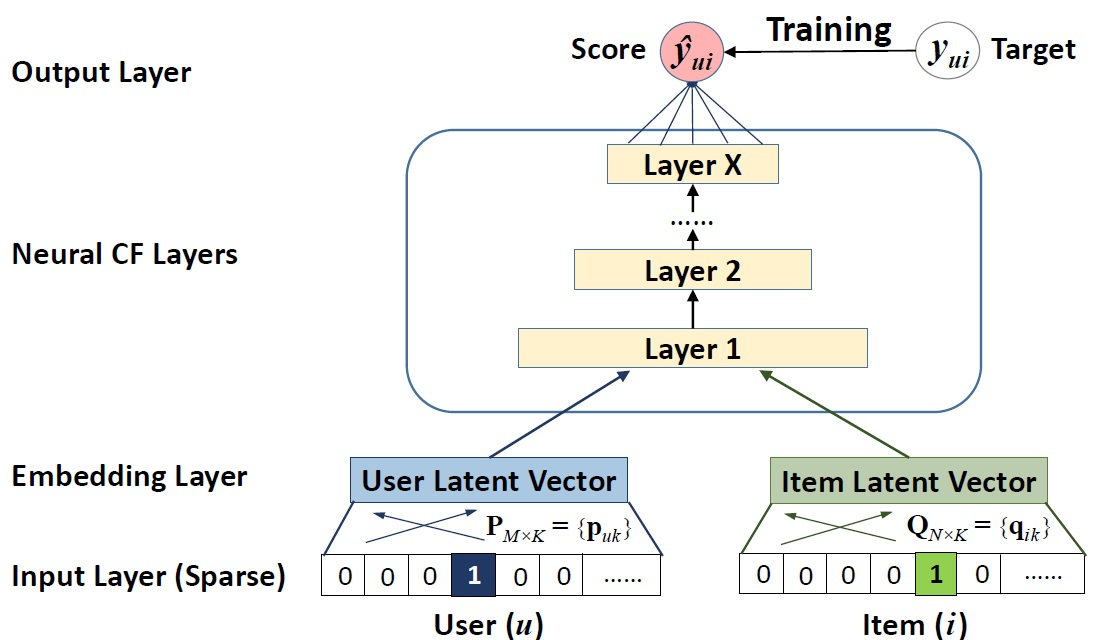
\includegraphics[width=\linewidth]{./img/ncf.jpg}
  \caption{NCF模型框架示意图。}
  \Description{NCF模型框架示意图。}
  \label{fig:ncf}
\end{figure}  

因此,构建一个对偶网络来建模用户和物品之间的双向交互是很自然的。 神经协同过滤(NCF)\cite{he2017neural} 就是这样一个框架,旨在捕捉用户和物品之间的非线性关系。图\ref{fig:ncf}展示了NCF架构。

让$s_u^{user}$和$s_i^{item}$分别表示辅助信息(例如用户配置文件和物品特征),或者只是用户$u$和物品$i$的one-hot标志。NCF的预测规则如下:

\begin{equation}
  \hat{r}_{u i}=f\left(U^{T} \cdot s_{u}^{u s e r}, V^{T} \cdot s_{i}^{i t e m} \mid U, V, \theta\right)
\end{equation}

其中函数$f(\cdot)$定义了多层感知器,$\theta$是这个网络的参数。用于预测显式评级的损失函数定义为加权平方误差:

\begin{equation}
  \mathcal{L}=\sum_{(u, i) \in \mathcal{O} \cup \mathcal{O}^{-}} w_{u i}\left(r_{u i}-\hat{r}_{u i}\right)^2
\end{equation}

\cite{wang2017item}将NCF模型扩展到跨域社交推荐,即向社交网络的潜在用户推荐信息域物品,并提出了一种神经社交协作排名推荐系统。

\textbf{CCCFNet} \cite{lian2017cccfnet} ,CCCFNet(跨域内容增强协同过滤神经网络)是另一个基于内容方法,对NCF的扩展模型。CCCFNet 的基本组合也是一个对偶网络(分别针对用户和物品)。它使用点积对最后一层中的用户-物品交互进行建模。 为了嵌入内容信息,作者进一步将双网的每个网络分解为两个组成部分:协同过滤因子(用户和物品潜在因子)和内容信息(用户对物品特征和物品特征的偏好)。 在这个基本模型上建立了一个多视图神经网络框架来执行跨域推荐。

\subsection{Using CNN in Content-based Methods}

\subsubsection{CNN for Image Feature Extraction}

Wang et al. \cite{wang2017your} 研究了视觉特征对兴趣点(POI)推荐的影响,并提出了一种视觉内容增强的POI推荐系统(VPOI)。VPOI 采用 CNN 提取图像特征。通过探索:(1)视觉内容和潜在用户因素之间的相互作用; (2) 视觉内容和潜在位置因素。Chu et al. \cite{chu2017hybrid} 在餐厅推荐中利用了视觉信息(例如餐厅的食物和家具的图像)的有效性。将 CNN 提取的视觉特征与文本表示联合输入到模型中以测试它们的效果。结果表明,视觉信息在一定程度上提高了性能,但并不显着。He et al. \cite{he2016vbpr} 通过将视觉特征(通过 CNN 学习)结合到矩阵分解中,设计了一种视觉贝叶斯个性化排名(VBPR)算法。

\subsubsection{CNN for Audio Feature Extraction} 

Van et al. \cite{van2013deep} 提出使用 CNN 从音乐信号中提取特征。卷积核和池化层允许在多个时间尺度上进行操作。 这种基于内容的模型可以缓解音乐推荐的冷启动问题(音乐没有被消费)。 让 $y'$ 表示 CNN 的输出,$y$表示从加权矩阵分解中学习到的物品潜在因子。 CNN 的目标是最小化$y$和$y'$之间的平方误差。 

\subsubsection{CNN for Text Feature Extraction} 

Shen et al. \cite{shen2016automatic} 建立了一个电子学习资源推荐模型。 它使用CNN从学习资源的文本信息中提取物品特征,例如学习资料的介绍和内容,进行推荐。

\section{Conclusion}

推荐系统在过去几十年中取得了重大进展,当时提出了许多基于内容的、协作过滤的方法,并且已经开发了若干应用。在本文中,我们回顾了当前若干种推荐方法,并介绍了机器学习提供的更好推荐功能的扩展。这些扩展包括改进的用户和物品建模、将上下文信息合并到推荐过程中、将推荐任务数学建模为统计问题并用机器学习方法解决等。我希望本文可以增深读者对于推荐系统中的机器学习理解。

%%
%% The next two lines define the bibliography style to be used, and
%% the bibliography file.
\bibliographystyle{ACM-Reference-Format}
\bibliography{references}
  
\end{document}
\endinput
%%
%% End of file `sample-sigconf.tex'.
